%%%%%%%%%%%%%%%%%%%%%%%%%%%%%%%%%%%%%%%%%%%%%%%%%
%------ LaTeX-Dokument f�r die gesamte Bachelorarbeit --------
%%%%%%%%%%%%%%%%%%%%%%%%%%%%%%%%%%%%%%%%%%%%%%%%%

%---- Header (mit Formateinstellugen) laden, Inputencoding pr�fen ------
%%%%%%%%%%%%%%%%%%%%%%%%%%%%%%%%%%%%%%%%%%%%%%%%%
%---- LaTeX-Header fuer Abschlussarbeiten, Prof. Thomas Goerne, Dez. 2012/Aug. 2013 ----
%%%%%%%%%%%%%%%%%%%%%%%%%%%%%%%%%%%%%%%%%%%%%%%%%

\documentclass[12pt,paper=A4,parskip=half, pointlessnumbers,bibtotoc,liststotoc,DIV=11,BCOR=1mm]{scrreprt}
% BCOR ist die Bindekorrektur (verlorener Rand am linken Blattrand)! Wert haengt von der Art der Heftung ab!!
% DIV ist eine Satzspiegeleinstellung von KOMA-Script / sccreprt.

\pagestyle{headings}

\usepackage[T1]{fontenc} % Font Encoding fuer europaeische Schriften mit Umlauten (Unterstuetzung der Worttrennung)
\usepackage{lmodern} % PostScript-Varianten der TeX Computer Modern-Schriften laden
\usepackage[english,ngerman]{babel} % Spracheinstellungen fuer Englisch und Neudeutsch laden

\usepackage{graphicx} % Grafikeinbindung (fuer .JPG, .JPEG, .PNG und .PDF, falls pdflatex benutzt wird)
\usepackage[table]{xcolor} % ermoeglicht farbige Schrift und farbige Tabellenzeilen
\definecolor{black}{gray}{0} % Umdefinition der Farbe black, falls noetig (0=schwarz, 1=weiss)
\definecolor{dblue}{rgb}{0.1,0.2,0.6} % Dunkelblau, fuer Hyperlinks
\definecolor{lgray}{gray}{0.9} % Hellgrau, fuer Tabellen (0=schwarz, 1=weiss)

\usepackage{booktabs} % fuer schoene Tabellen

\usepackage[round,authoryear]{natbib} % Literaturverweise mit Name/Jahreszahl in runden Klammern
\bibpunct[:\,]{(}{)}{,}{a}{}{,~}  % Feinformatierung der Natbib-Zitierweise

\usepackage[hyphens]{url}
\usepackage[colorlinks=true,linkcolor=black,citecolor=dblue,urlcolor=dblue]{hyperref} 
\usepackage{hyperref}  
% die Pakete url und hyperref ermoeglichen anklickbare URLs im Quellenverzeichnis in definierter Farbe, 
% sie ermoeglichen den Zeilenumbruch bei langen URLs, und sie erzeugen Hyperlinks (Farbe s.o.) 
% zwischen Quellenverweis und Quellenverzeichnis sowie zwischen label und ref im PDF-Dokument

% Fonteinstellungen fuer Bildunterschriften: Unterschrift serifenlos, "Abbildung" fett (bfseries = bold face series)
\setkomafont{captionlabel}{\sffamily\bfseries}
\setkomafont{caption}{\sffamily}

%---- eigene Packages ------
%\usepackage[usenames,dvipsnames,svgnames,table]{xcolor}
\usepackage{acronym}
\usepackage[latin1]{inputenc} % Inputencoding f�r PC/Win
\usepackage{tikz}
\usepackage{amsmath, amssymb}
\usepackage{mathtools}
\usepackage{pgffor}
\usepackage{varwidth}
\newcommand\Umbruch[2][3cm]{\begin{varwidth}{#1}\centering#2\end{varwidth}}
\usetikzlibrary{shapes,snakes}
\usetikzlibrary{positioning}
\usepgflibrary{arrows}
\usepackage{caption}
\usepackage{pgfplots}
\usepackage{subcaption}
\usepackage{xcolor}
\usepackage{listings}


\renewcommand{\thefootnote}{\roman{footnote}}
\newcommand{\net}{\operatorname{net}}


\colorlet{punct}{red!60!black}
\definecolor{background}{HTML}{EEEEEE}
\definecolor{delim}{RGB}{20,105,176}
\colorlet{numb}{magenta!60!black}

\lstdefinelanguage{json}{
    %basicstyle=\footnotesize\ttfamily,
    %numbers=left,
    %numberstyle=\scriptsize,
    %stepnumber=1,
    %numbersep=8pt,
    %showstringspaces=false,
    sensitive=false,
    %breaklines=true,
    %frame=lines,
    %backgroundcolor=\color{background},
    escapeinside={...a}{a...},
    literate=
     *{0}{{{\color{numb}0}}}{1}
      {1}{{{\color{numb}1}}}{1}
      {2}{{{\color{numb}2}}}{1}
      {3}{{{\color{numb}3}}}{1}
      {4}{{{\color{numb}4}}}{1}
      {5}{{{\color{numb}5}}}{1}
      {6}{{{\color{numb}6}}}{1}
      {7}{{{\color{numb}7}}}{1}
      {8}{{{\color{numb}8}}}{1}
      {9}{{{\color{numb}9}}}{1}
      {:}{{{\color{punct}{:}}}}{1}
      {,}{{{\color{punct}{,}}}}{1}
      {\{}{{{\color{delim}{\{}}}}{1}
      {\}}{{{\color{delim}{\}}}}}{1}
      {[}{{{\color{delim}{[}}}}{1}
      {]}{{{\color{delim}{]}}}}{1},
}

\definecolor{lightgray}{rgb}{.9,.9,.9}
\definecolor{darkgray}{rgb}{.4,.4,.4}
\definecolor{purple}{rgb}{0.65, 0.12, 0.82}

\lstdefinelanguage{JavaScript}{
  keywords={typeof, new, true, false, catch, function, return, null, catch, switch, var, if, in, while, do, else, case, break},
  keywordstyle=\color{blue}\bfseries,
  ndkeywords={class, export, boolean, throw, implements, import, this},
  ndkeywordstyle=\color{darkgray}\bfseries,
  identifierstyle=\color{black},
  sensitive=false,
  comment=[l]{//},
  morecomment=[s]{/*}{*/},
  commentstyle=\color{purple}\ttfamily,
  stringstyle=\color{red}\ttfamily,
  morestring=[b]',
  escapeinside={...a}{a...},
  morestring=[b]"
}

\lstset{
   language=JavaScript,
   backgroundcolor=\color{lightgray},
   extendedchars=true,
   basicstyle=\footnotesize\ttfamily,
   showstringspaces=false,
   showspaces=false,
   numbers=left,
   numberstyle=\footnotesize,
   numbersep=9pt,
   tabsize=2,
   breaklines=true,
   showtabs=false,
   captionpos=b
}



%------------------------------------------------------------------------------------------------------------------
%------ Eigenstaendigkeitserklaerung im gerahmten Kasten (parbox in einer framebox) ------
%------------------------------------------------------------------------------------------------------------------

\newcommand{\eigen}{
\setlength{\fboxsep}{2ex}
\setlength{\fboxrule}{0.8pt} 
% Einstellungen fuer Rahmenabstand und Rahmendicke der Framebox
\begin{center}
	\fbox{
		\parbox{0.8\linewidth}{
		Ich versichere, die vorliegende Arbeit selbstst\"andig ohne fremde Hilfe verfasst 
		und keine anderen Quellen und Hilfsmittel als die angegebenen benutzt zu haben. 
		Die aus anderen Werken w\"ortlich entnommenen Stellen oder dem Sinn nach 
		entlehnten Passagen sind durch Quellenangaben eindeutig kenntlich gemacht.
		\par\bigskip\bigskip\bigskip\bigskip
		\hspace*{0.8cm}Ort, Datum \hfill \vorname~\nachname\hspace*{0.8cm}
		}
	}
\end{center}
}

%%%%%%%%%%%%%%%%%%%%%%%%%%%%%%%%%%%%%%%%%%%%%%%%%
\usepackage[latin1]{inputenc} % Inputencoding f�r PC/Win


%------------------------ Titelblatt-Layout laden ----------------------------------
%%%%%%%%%%%%%%%%%%%%%%%%%%%%%%%%%%%%%%%%%%%%%%%%%
%------ LaTeX-Titelblatt fuer Bachelorarbeiten, Prof. Thomas Goerne, Dezember 2012 -------
%------------------------------------------------------------------------------------------------------------------
%--------------------------------- Deklarationen fuer die Titelseite  --------------------------------------
%%%%%%%%%%%%%%%%%%%%%%%%%%%%%%%%%%%%%%%%%%%%%%%%%

\title{\titel\\[2ex]
\LARGE Bachelor-Thesis\\
\large zur Erlangung des akademischen Grades B.Sc.\\[1.5ex]
\LARGE \vorname~\nachname\\[0.5ex] 
\large \matrikelnummer
}

\author{\unitlength1mm
\large\raisebox{-1ex}{
\includegraphics[width=4em]{HAW_wuerfel}}\hspace{1ex}
\parbox[b]{11.2cm}{\sffamily\large%
Hochschule f\"ur Angewandte Wissenschaften Hamburg\\[-0.2ex]
Fakult\"at Design, Medien und Information\\[-0.2ex]
Department Medientechnik
}\\[6ex]
\sffamily\large Erstpr\"ufer: \erstpruef\\[0.5ex]
\sffamily\large Zweitpr\"ufer: \zweitpruef}

%%%%%%%%%%%%%%%%%%%%%%%%%%%%%%%%%%%%%%%%%%%%%%%%%
%\input{hawmt-master-titelblatt}

%---------------------------- Titeldefinitionen --------------------------------------

\newcommand{\vorname}{Xuan Linh}
\newcommand{\nachname}{Do}
\newcommand{\matrikelnummer}{218196}

\newcommand{\titel}{Realisierung eines interaktiven k�nstlichen neuronalen Netzwerks in Javascript mit spielerischen Elementen
%\\[0.2ex]\Large Untertitel Untertitel Untertitel Untertitel
}			
\newcommand{\erstpruef}{Prof. Edmund Weitz}
\newcommand{\zweitpruef}{Prof. Andreas Pla�}

\date{vorl�ufige Fassung vom \today}   % praktisch f�r Vorab-Versionen. 
%\date{\sffamily Hamburg, 2. 2. 2020}  % Abgabedatum!

%--------------------------------------------------------------------------------------
%----------------------------- hier gehts los! --------------------------------------
%--------------------------------------------------------------------------------------

\begin{document}
\selectlanguage{ngerman}
\maketitle           % Titelseite erzeugen
\tableofcontents % Inhaltsverzeichnis erzeugen
\clearpage          % Seitenumbruch


%------------ Zusammenfassung / Abstract ------------------

\thispagestyle{empty}
\selectlanguage{english}
\section*{\centering\abstractname}

English
 
 
\selectlanguage{ngerman}
\section*{\centering\abstractname}
Diese Arbeit ist eine Fortf�hrung der von Finn Ole Koenecke angefertigten Bachelorarbeit mit dem Titel "Realisierung eines interaktiven k�nstlichen neuronalen Netzwerks" aus dem Jahre 2016. Im Rahmen seiner Arbeit wurde ein Programm geschrieben, indem der Anwender interaktiv die Arbeitsweise und Strukturen von neuronalen Netzen visualisieren und erlernen kann. Das Programm ist so aufgebaut, dass die graphische Oberfl�che �ber den Browser und die Rechenarbeit f�r das neuronale Netz im Hintergrund �ber einen Server l�uft.
Ziel dieser Bachelorarbeit ist es, dieses Programm komplett in Javascript, HTML und CSS zu portieren, sodass dieser auch ohne einen Server im Browser l�uft. Zudem soll das Programm so erweitert werden, dass das neuronale Netz spielerisch eingesetzt werden kann.
 

%--------------------------- Text -------------------------------

%% !TEX root = BachelorthesisNeu.tex
%%%%%%%%%%%%%%%%%%%%%%%%%%%%%%%%%%%%%%%%%%%%%%%%%%
%---- LaTeX-Header fuer Abschlussarbeiten, Prof. Thomas Goerne, Dez. 2012/Aug. 2013 ----
%%%%%%%%%%%%%%%%%%%%%%%%%%%%%%%%%%%%%%%%%%%%%%%%%

\documentclass[12pt,paper=A4,parskip=half, pointlessnumbers,bibtotoc,liststotoc,DIV=11,BCOR=1mm]{scrreprt}
% BCOR ist die Bindekorrektur (verlorener Rand am linken Blattrand)! Wert haengt von der Art der Heftung ab!!
% DIV ist eine Satzspiegeleinstellung von KOMA-Script / sccreprt.

\pagestyle{headings}

\usepackage[T1]{fontenc} % Font Encoding fuer europaeische Schriften mit Umlauten (Unterstuetzung der Worttrennung)
\usepackage{lmodern} % PostScript-Varianten der TeX Computer Modern-Schriften laden
\usepackage[english,ngerman]{babel} % Spracheinstellungen fuer Englisch und Neudeutsch laden

\usepackage{graphicx} % Grafikeinbindung (fuer .JPG, .JPEG, .PNG und .PDF, falls pdflatex benutzt wird)
\usepackage[table]{xcolor} % ermoeglicht farbige Schrift und farbige Tabellenzeilen
\definecolor{black}{gray}{0} % Umdefinition der Farbe black, falls noetig (0=schwarz, 1=weiss)
\definecolor{dblue}{rgb}{0.1,0.2,0.6} % Dunkelblau, fuer Hyperlinks
\definecolor{lgray}{gray}{0.9} % Hellgrau, fuer Tabellen (0=schwarz, 1=weiss)

\usepackage{booktabs} % fuer schoene Tabellen

\usepackage[round,authoryear]{natbib} % Literaturverweise mit Name/Jahreszahl in runden Klammern
\bibpunct[:\,]{(}{)}{,}{a}{}{,~}  % Feinformatierung der Natbib-Zitierweise

\usepackage[hyphens]{url}
\usepackage[colorlinks=true,linkcolor=black,citecolor=dblue,urlcolor=dblue]{hyperref} 
\usepackage{hyperref}  
% die Pakete url und hyperref ermoeglichen anklickbare URLs im Quellenverzeichnis in definierter Farbe, 
% sie ermoeglichen den Zeilenumbruch bei langen URLs, und sie erzeugen Hyperlinks (Farbe s.o.) 
% zwischen Quellenverweis und Quellenverzeichnis sowie zwischen label und ref im PDF-Dokument

% Fonteinstellungen fuer Bildunterschriften: Unterschrift serifenlos, "Abbildung" fett (bfseries = bold face series)
\setkomafont{captionlabel}{\sffamily\bfseries}
\setkomafont{caption}{\sffamily}

%---- eigene Packages ------
%\usepackage[usenames,dvipsnames,svgnames,table]{xcolor}
\usepackage{acronym}
\usepackage[latin1]{inputenc} % Inputencoding f�r PC/Win
\usepackage{tikz}
\usepackage{amsmath, amssymb}
\usepackage{mathtools}
\usepackage{pgffor}
\usepackage{varwidth}
\newcommand\Umbruch[2][3cm]{\begin{varwidth}{#1}\centering#2\end{varwidth}}
\usetikzlibrary{shapes,snakes}
\usetikzlibrary{positioning}
\usepgflibrary{arrows}
\usepackage{caption}
\usepackage{pgfplots}
\usepackage{subcaption}
\usepackage{xcolor}
\usepackage{listings}


\renewcommand{\thefootnote}{\roman{footnote}}
\newcommand{\net}{\operatorname{net}}


\colorlet{punct}{red!60!black}
\definecolor{background}{HTML}{EEEEEE}
\definecolor{delim}{RGB}{20,105,176}
\colorlet{numb}{magenta!60!black}

\lstdefinelanguage{json}{
    %basicstyle=\footnotesize\ttfamily,
    %numbers=left,
    %numberstyle=\scriptsize,
    %stepnumber=1,
    %numbersep=8pt,
    %showstringspaces=false,
    sensitive=false,
    %breaklines=true,
    %frame=lines,
    %backgroundcolor=\color{background},
    escapeinside={...a}{a...},
    literate=
     *{0}{{{\color{numb}0}}}{1}
      {1}{{{\color{numb}1}}}{1}
      {2}{{{\color{numb}2}}}{1}
      {3}{{{\color{numb}3}}}{1}
      {4}{{{\color{numb}4}}}{1}
      {5}{{{\color{numb}5}}}{1}
      {6}{{{\color{numb}6}}}{1}
      {7}{{{\color{numb}7}}}{1}
      {8}{{{\color{numb}8}}}{1}
      {9}{{{\color{numb}9}}}{1}
      {:}{{{\color{punct}{:}}}}{1}
      {,}{{{\color{punct}{,}}}}{1}
      {\{}{{{\color{delim}{\{}}}}{1}
      {\}}{{{\color{delim}{\}}}}}{1}
      {[}{{{\color{delim}{[}}}}{1}
      {]}{{{\color{delim}{]}}}}{1},
}

\definecolor{lightgray}{rgb}{.9,.9,.9}
\definecolor{darkgray}{rgb}{.4,.4,.4}
\definecolor{purple}{rgb}{0.65, 0.12, 0.82}

\lstdefinelanguage{JavaScript}{
  keywords={typeof, new, true, false, catch, function, return, null, catch, switch, var, if, in, while, do, else, case, break},
  keywordstyle=\color{blue}\bfseries,
  ndkeywords={class, export, boolean, throw, implements, import, this},
  ndkeywordstyle=\color{darkgray}\bfseries,
  identifierstyle=\color{black},
  sensitive=false,
  comment=[l]{//},
  morecomment=[s]{/*}{*/},
  commentstyle=\color{purple}\ttfamily,
  stringstyle=\color{red}\ttfamily,
  morestring=[b]',
  escapeinside={...a}{a...},
  morestring=[b]"
}

\lstset{
   language=JavaScript,
   backgroundcolor=\color{lightgray},
   extendedchars=true,
   basicstyle=\footnotesize\ttfamily,
   showstringspaces=false,
   showspaces=false,
   numbers=left,
   numberstyle=\footnotesize,
   numbersep=9pt,
   tabsize=2,
   breaklines=true,
   showtabs=false,
   captionpos=b
}



%------------------------------------------------------------------------------------------------------------------
%------ Eigenstaendigkeitserklaerung im gerahmten Kasten (parbox in einer framebox) ------
%------------------------------------------------------------------------------------------------------------------

\newcommand{\eigen}{
\setlength{\fboxsep}{2ex}
\setlength{\fboxrule}{0.8pt} 
% Einstellungen fuer Rahmenabstand und Rahmendicke der Framebox
\begin{center}
	\fbox{
		\parbox{0.8\linewidth}{
		Ich versichere, die vorliegende Arbeit selbstst\"andig ohne fremde Hilfe verfasst 
		und keine anderen Quellen und Hilfsmittel als die angegebenen benutzt zu haben. 
		Die aus anderen Werken w\"ortlich entnommenen Stellen oder dem Sinn nach 
		entlehnten Passagen sind durch Quellenangaben eindeutig kenntlich gemacht.
		\par\bigskip\bigskip\bigskip\bigskip
		\hspace*{0.8cm}Ort, Datum \hfill \vorname~\nachname\hspace*{0.8cm}
		}
	}
\end{center}
}

%%%%%%%%%%%%%%%%%%%%%%%%%%%%%%%%%%%%%%%%%%%%%%%%%
%
%\begin{document}
%%______________________________________



\chapter{Einleitung}\label{c:einleitung}
\section{Motivation}
Bei vielen Aufgaben ist es von gro�em Vorteil auf technische Hilfsmittel zuzugreifen, da sie so erheblich schneller gel�st werden k�nnen. Zum Beispiel kann f�r die Berechnung komplexerer Rechenaufgaben der Taschenrechner genutzt werden. Jedoch soll nicht au�er Acht gelassen werden, dass ein Rechner darauf beschr�nkt ist, nur eine begrenzte Anzahl von Aufgaben erledigen zu k�nnen. Der Mensch kann sich dagegen mit seiner Flexibilit�t und Vielseitigkeit auszeichnen. Zudem gibt es immer noch viele Aufgaben, in denen der Computer dem Menschen deutlich unterlegen ist. \emph{\glqq Wahrnehmung und Erkennen, Lernen und Speichern von Informationen, Anpassung an die Umwelt, Steuerung von Verhalten sowie Kreativit�t sind Leistungen des menschlichen Nervensystems, die Maschinen bisher erst in Ans�tzen in der Lage sind nachzuahmen.\grqq} \citep[S. 119]{kramer} 

Zu den Ans�tzen, die im Zitat genannten Fertigkeiten auch dem Computer zu erm�glichen, z�hlen unter anderem \ac{KNN}. Dank der j�ngsten technischen Fortschritte in diesem Bereich k�nnen immer mehr komplexere Aufgaben auch vom Computer gel�st werden. Im Bereich der Spiele k�nnen sie zum Beispiel beim Jump'n'Run-Videospiel \emph{Super Mario World} eingesetzt werden, wie der Youtuber \emph{SethBling} in einem seiner Videos zeigt \citep{sethBling}. Zudem gibt es nicht nur Computerprogramme, die imstande sind, mithilfe von \ac{KNN} die besten Spieler in komplexen Spielen zu schlagen, in denen alle Informationen offen gelegt sind wie beim Brettspiel \emph{Go}. Auch bei \emph{Texas Hold'em}, einer Variante des Kartenspiels Poker, die aufgrund der verdeckten Karten auf die Intuition und Gl�ck aufbauen, haben \ac{KNN} dazu beigetragen, dass professionelle Spieler von einem Computerprogramm geschlagen werden konnten \citep{riley}. Die Abbildung \ref{einsatzKNN} zeigt, in welchen Bereichen \ac{KNN} noch eingesetzt werden k�nnen. 

\begin{figure}[htp]     % h=here, t=top, b=bottom, p=page
\centering
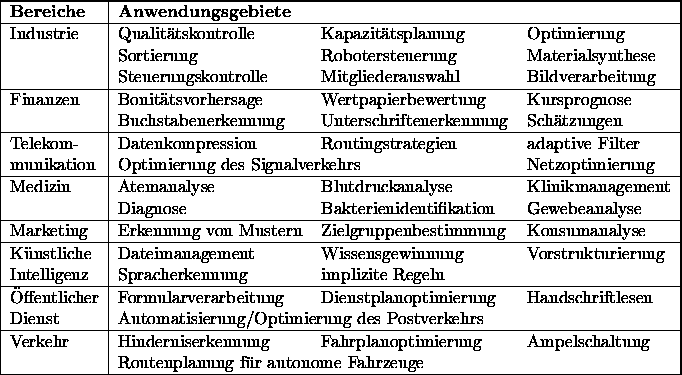
\includegraphics[width=0.8\textwidth]{../einleitung/bilder/einsatzKNN} 
% Bilddatei aus dem Unterverzeichnis bilder holen, skalieren auf 0.8*Satzspiegel
\caption{Anwendungsgebiete f�r den Einsatz von KNN, entnommen aus \url{http://vieta.math.tu-cottbus.de/~kolb/ml-nn/node10.html}}\label{einsatzKNN}
\end{figure}

\section{Begriffsdefinition}
\ac{KNN} sind die stark abstrahierte, technische Umsetzung der biologischen neuronalen Netze des menschlichen Gehirns. Mithilfe des Wissens �ber die Struktur und Funktionsweise vom Nervensystem k�nnen die biologischen Prinzipien der Informationsverarbeitung als systematisches Modell f�r den Rechner �bertragen werden.

\section{Zielsetzung}
Das Hauptziel dieser Arbeit ist es, dem Leser und Anwender einen leichten Einstieg in das Thema \ac{KNN} und deren Einsatzm�glichkeiten zu bieten. Damit wird dasselbe Ziel verfolgt, das schon Herr Koenecke mit seiner Arbeit hatte. Mit dem theoretischen Teil soll eine gewisse Wissensbasis �ber \ac{KNN} geschaffen werden. Beim praktischen Teil kann der Anwender mithilfe eines Programms, das durch den theoretischen Teil erworbene Wissen interaktiv veranschaulichen und verfestigen. Folgender Textauszug aus Herr Koeneckes Arbeit zeigt, was die Anforderungen an seinem geschriebenen Programm sind:

\emph{\glqq Die Grundidee besteht daraus, ein neuronales Netz zu implementieren, dessen Abl�ufe zu jeder Zeit angehalten und dessen interner Status eingesehen werden kann. �ber eine grafische Oberfl�che ist es dann m�glich, diese Funktionen aufzurufen, um das Netzwerk zu bedienen. W�hrenddessen k�nnen die internen Mechanismen beobachtet werden. So kann
ein Anwender testweise Eingaben t�tigen, deren Auswirkungen beobachten und daraus
Schl�sse ziehen. Die Interna des Netzwerks werden transparent. Anhand von bekannten
und interessanten Problemen kann sich so auch ein unerfahrener Nutzer die Funktionsweise
neuronaler Netze erschlie�en.\grqq} \citep[S. 7]{koenecke}

Weitestgehend sind die Anforderungen mit dem urspr�nglichen Programm erreicht worden. Ausgehend von diesem Programm als Basis sollen f�r diese Arbeit zwei gr��ere �nderungen stattfinden:


\begin{enumerate}\setlength{\itemsep}{0ex}
\item \emph{Portieren seines Programms komplett in Javascript, HTML und CSS}: Dies setzt voraus, dass die Berechnungen f�r das \ac{KNN} nicht mehr wie bisher im Hintergrund �ber einen Server laufen, sondern komplett lokal im Browser in Javascript durchgef�hrt werden. 
Von der Portierung ist zu erwarten, dass das Programm zwar nicht so schnell wie das urspr�ngliche Programm laufen wird, aber dennoch performant genug, dass es sich fl�ssig in einem aktuellen Browser benutzen l�sst.
\item \emph{�nderung des User Interfaces durch Hinzuf�gen spielerischer Elemente}: Die graphische Oberfl�che des Programms soll ver�ndert werden, sodass spielerische Interaktionen m�glich sind. Dabei ist es wichtig, dass das N�herbringen der Grundlagen von KNN immer noch im Vordergrund des Programms stehen soll. Daher sind die Ver�nderungen am Programm vor allem als Erweiterungen zu betrachten. Die Idee f�r die Erweiterungen fokussiert sich dabei auf den letzten Satz der oben von Herr Koenecke zitierten Textpassage, also die M�glichkeit anhand bekannter Probleme die Arbeitsweise \ac{KNN} zu erlernen. Im urspr�nglichen Programm ist der Anwender noch dazu gezwungen, sich die Probleme selbst herauszusuchen oder auszudenken. Um ihm diesen Schritt zu ersparen, soll es zus�tzlich eine Option vom Programm geben, anhand gestellter Aufgaben die Probleme kennenzulernen. Zum L�sen dieser Aufgaben, muss der Anwender die passenden Konfigurationen des \ac{KNN} vornehmen. So erh�lt der Anwender die M�glichkeit spielerisch zu erlernen, wie und wozu \ac{KNN} eingesetzt werden k�nnen.
\end{enumerate}

\section{Anmerkungen im Bezug auf Koeneckes Arbeit}
Zum Lesen dieser Arbeit soll keine zwingende Voraussetzung sein, Herrn Koeneckes Bachelorthesis durchzulesen. Daher werden sich einige �berschneidungen und Verweise zu Koeneckes Arbeit finden. Dies l�sst sich sowieso nicht komplett aufgrund der Tatsache vermeiden, dass diese Arbeit und der dazugeh�rige praktische Teil auf Grundlage seiner Arbeit und Anwendung entstanden ist. Die gr��ten �berschneidungen finden sich vor allem in den Kapiteln 2 - 5, in denen die Theorie behandelt wird, die mit der K�nstlichen Intelligenz und den \ac{KNN} in Verbindung stehen \citep[nachzulesen in seiner Thesis auf den Seiten S. 4-5 sowie 11-32]{koenecke}. Im Unterschied zu seiner Arbeit wurde die Theorie der KNN auf mehr Kapitel unterteilt und eine andere Strukturierung ausgew�hlt, mit dem Ziel eine bessere �bersicht �ber das Thema zu bieten. Ob dieser Weg wirklich der bessere ist, h�ngt im Grunde genommen vom Leser ab. Bevorzugt er es lieber kompakt in einem Kapitel sich die Theorie anzueignen, w�re die bessere Entscheidung sich Herr Koeneckes Arbeit durchzulesen. M�chte er lieber st�ckchenweise sich �ber verschiedene Kapitel die Theorie aneignen, kann diese Arbeit die bessere Wahl sein. 
%Vor allem richten sich diese Kapitel also an Leser, die seine Bachelorthesis noch nicht gelesen haben, nur wenig Wissen �ber \ac{KNN} haben und sich mit einem leichten Einstieg in das Thema zufrieden geben k�nnen. Genauso empfehlenswert sind sie f�r Leser, die ihr Wissen �ber \ac{KNN} noch einmal auffrischen wollen.

\section{Struktur dieser Arbeit}
\textcolor{red}{KOMMT AM ENDE}

\chapter{Grundlagen}\label{cGrundlagen} 
In diesem Kapitel soll eine grundlegende Wissensbasis zur Einordnung der Begriffe \ac{KI}, Maschinelles Lernen, Deep Learning und \ac{KNN} geschaffen werden. So kommt es bei Laien h�ufiger zu Verwechslungen dieser Begriffe, deswegen sollen in diesem Kapitel genauer auf sie eingegangen werden, bevor im Kapitel \ref{cKnn} der tiefere Einblick in die Theorie der \ac{KNN} erfolgt. Auf diese Weise l�sst sich besser verstehen, was \ac{KNN} sind und was sie nicht sind, f�r welchen Bereich sie eine Bedeutung spielen und wie sie in der Informatik einzuordnen sind. Es wird sich zeigen, dass das Thema \ac{KI} so breit gef�chert ist, dass f�r die Arbeit nur ein oberfl�chlicher Einschnitt in das Thema erfolgt. So werden vor allem die Grundlagen behandelt, die f�r die Thematik der \ac{KNN} und das im Rahmen der Bachelorthesis geschriebene Programm von Bedeutung sind.
Den Lesern, die tiefer in die Materie gehen m�chten, steht es nach der Einf�hrung mithilfe dieser Bachelorthesis offen, sich danach anderweitig �ber das Thema \ac{KI} zu informieren. 

\section{K�nstliche Intelligenz}

\subsection{Begriffserkl�rung}
Ob der Mensch ein Lebewesen oder eine Maschine f�r intelligent h�lt oder nicht, beruht meist auf seine relativ gute Intuition. So beurteilt er wie ausgepr�gt die kognitiven F�higkeiten sind, um sich an ungewohnte Situationen anzupassen. Aus wissenschaftlicher Sicht gibt es jedoch keine allgemein g�ltige Definition f�r den Begriff \emph{Intelligenz} \citep[S. 139]{rimscha}. \emph{\glqq Befragt man heute 20 Intelligenzforscher nach einer Definition, erh�lt man 20 unterschiedliche Antworten\grqq}, ist die Aussage von Thomas Gr�ter, einem Arzt und Sachbuchautor, der f�r die Neurophysiologie forschte \citep[S. 139]{hillmann}. Dass der Begriff Intelligenz schwer zu definieren ist, zeigt ebenfalls, wie schwierig es ist, die \ac{KI} zu definieren. Grob formuliert wird unter \ac{KI} \emph{die Nachbildung menschlicher Intelligenz durch Maschinen} verstanden(\textcolor{red}{Quelle nochmal raussuchen :P}). Dies betrifft auch die menschliche Wahrnehmung und das menschliche Handeln.

\subsection{Turing Test}
Um festzustellen, ob eine Maschine dem Anspruch der \ac{KI} gen�gt, hat Alan M. Turing als Vorschlag in seinem Paper \citep{turing} den nach ihm benannten Turing-Test ausgedacht. �ber l�ngere Zeit kommuniziert ein Mensch als Tester parallel mit zwei Gespr�chspartnern. Bei dem einen Gespr�chspartner handelt es sich um einen Menschen, bei dem anderen um eine Maschine. Die Kommunikation erfolgt ohne Sicht- und H�rkontakt (beispielsweise �ber ein Chat-Programm). Sowohl Mensch als auch Maschine versuchen den Tester zu �berzeugen, dass sie denkende Menschen sind. Kann der Tester nach der Unterhaltung nicht bestimmen, welcher von den Gespr�chspartnern die Maschine ist, gilt der Test als bestanden und die Maschine kann als intelligent bezeichnet werden. 

Bisherige Versuche diesen Test zu bestehen, gab es bereits mit Programmen wie \emph{ELIZA} (1966) oder dem Chatbot \emph{Eugene Goostman} (2014). Doch bei keinem dieser Versuche kann von Experten wirklich �berzeugt best�tigt werden, dass sie den Turing Test bestanden haben. Und trotz der intensiven Forschung im Bereich der \ac{KI} wird mit gro�er Wahrscheinlichkeit auch in absehbarer Zeit dies nicht passieren. 

\subsection{Starke und schwache \ac{KI}}
Aufgrund der Komplexit�t der \ac{KI} ist die Idee gekommen, eine Unterscheidung vorzunehmen \citep{russell-norvig}. Zum einen die \emph{starke \ac{KI}}, die dem Menschen ebenb�rtig ist und dazu imstande ist, komplexe kognitive Aufgaben autonom zu bew�ltigen, die sonst nur der Mensch l�sen kann. Zum anderen die \emph{schwache \ac{KI}}, die sich auf die L�sung der Probleme konzentriert, die konkretisiert und stark eingrenzt sind. In dieser Arbeit wird es ausschlie�lich um die L�sungsans�tze von Problemen aus dem Gebiet der schwachen \ac{KI} gehen. Beispielsweise z�hlen in das Gebiet der schwachen \ac{KI} Suchmaschinen, Spracherkennung und Bilderkennung, in denen in letzter Zeit beachtliche Erfolge erzielt werden konnten. Als Beispiele sind das 2014 von Amazon ver�ffentlichte, sprach-gesteuerte Ger�t Amazon Echo oder die Internet-Suchmaschine Google zu nennen. Sowohl die starke als auch die schwache \ac{KI} haben gemeinsam, dass bei beidem das Maschinelle Lernen eine immer gr��ere Bedeutung spielt. 

\section{Maschinelles Lernen}
\subsection{Begriffserkl�rung}
Beim Maschinellen Lernen (englisch: \emph{artificial intelligence - AI}) geht es um den Gewinn von Informationen und Wissen aus Erfahrung in Form von konkreten Beispieldaten \citep[ S. 143]{rimscha}. Im Gegensatz zur \emph{Symbolischen \ac{KI}} l�st der Computer also die Aufgabe nicht durch eine ihm vorher vorgegebene L�sungsvorschrift, sondern muss sich die L�sungsvorschrift selbst ableiten. Dadurch ist es f�r ihn auch m�glich, L�sungen f�r neue oder unbekannte Probleme zu finden. 

Die abgeleitete L�sungsvorschrift und damit die Ergebnisse dieser sind nur so gut, wie die Beispieldaten. Wenn die Beispieldaten nur einen bestimmten Bereich des Problems abdecken, aber nicht das Ganze, so werden die Daten als schlecht betrachtet. Um zu verdeutlichen, was damit gemeint ist, folgendes Beispiel: Es soll das Konsumverhalten von Pizza untersucht werden und es handelt sich bei den Testpersonen zuf�lligerweise um welche, die auf Di�t sind. Die Repr�sentativit�t der daraus entstehenden Ergebnisse wird unter diesen Bedingungen stark in Zweifel genommen werden k�nnen. Ebenfalls f�hren zu wenige zur Verf�gung stehende Daten zu schlechten Ergebnisse, deswegen k�nnen diese auch als schlechte Beispieldaten betrachtet werden. 

\subsection{Prinzip und Verfahren}

Das Maschinelle Lernen funktioniert im Grunde �hnlich wie das menschliche Lernen \citep{manhart}. So wird versucht, anhand der gegebenen Daten diese intelligent miteinander zu verkn�pfen, durch Ausprobieren und Abgleichen bestimmte Zusammenh�nge sowie Ergebnisse zu erschlie�en und anhand dieser Vorhersagen treffen zu k�nnen. Bei der Erkennung von Objekten auf Bildern lernt ein Mensch im Kindesalter zum Beispiel wie ein Hund aussieht, indem ihm Beispielbilder gezeigt werden, mit dem Hinweis, dass es sich um Hunde handelt. Auch beim Maschinellen Lernen f�ttert und trainiert der Programmierer das Lernprogramm mit Informationen in Form von Daten. Bei jeder Datei gibt er zus�tzlich an, ob es sich um einen Hund handelt oder nicht. Je mehr Beispieldaten das Programm bekommt, desto besser kann er unterscheiden, auf welchen Bildern Hunde zu sehen sind und auf welchen nicht. 

Um aus den Beispieldaten Wissen zu gewinnen, gibt es verschiedene Verfahren, die mathematische und statistische Algorithmen und Methoden verwenden. Davon nennenswerte w�ren zum Beispiel Entscheidungsb�ume, Reinforcement Learning, Genetische/Evolution�re Algorithmen, das Bayes'sche Lernen, der Monte Carlo Tree Search oder \ac{KNN}.\footnote{Die beiden letztgenannten Verfahren wurden unter anderem auch in dem von der Google-Tochter \emph{Deepmind} stammendem Programm \emph{Alpha Go} verwendet, der in der Lage war, im Mai 2017 den damaligen Weltranglistenersten \emph{Ke Jie} in drei von drei Go-Partien zu schlagen \citep{wunderlich}. Das ist insofern beachtlich, dass Go als sehr komplexes Brettspiel gilt. So bietet es mit ca. \( 2,08 \cdot 10^{170} \) m�glichen Stellungen sogar mehr als Schach mit $10^{43}$ m�glichen Stellungen.} Die verschiedenen Verfahren sind dabei nicht v�llig getrennt voneinander zu betrachten. Beispielsweise finden sich �berschneidungen zwischen genetischen Algorithmen und \ac{KNN}. Zudem sei zu erw�hnen, dass f�r die L�sung eines Problems auch oftmals nicht nur einer der Verfahren verwendet wird, sondern eine Kombination der verschiedenen Verfahren.

\section{Einordnung der KNN}
Anhand der vorherigen Erl�uterungen sollte nun klar zu unterscheiden sein, wie die verschiedenen Begriffe im Zusammenhang stehen. So sind \ac{KNN} ein Unterthema des Maschinellen Lernens, das wiederum ein Unterthema der \ac{KI} ist. Die Abbildung \ref{funktionLayer} soll diesen Zusammenhang veranschaulichen. 


\begin{figure}[!htb]
  \centering
	\begin{tikzpicture}
	\node[ellipse, minimum width=430, minimum height=180, thick, draw=black] (AI) at (0,10) {};
	\node[ellipse, minimum width=320, minimum height=150, thick, draw=black] (ML) at (-1.5,10) {};
	\node[ellipse, minimum width=200, minimum height=120, thick, draw=black] (NN) at (-3,10) {};
	\node[ellipse, minimum width=100, minimum height=90, thick, draw=black] (DL) at (-4.5,10) {};
	\node[above right = -1.7 and 0.3 of ML, text width=5cm,align=center, font=\large](){K�nstliche \\Intelligenz};
	\node[above right = -1.4 and -0.3 of NN, text width=5cm,align=center, font=\large](){Maschinelles \\Lernen};
	\node[above right = -0.1 and -0.9 of DL, text width=5cm,align=center, font=\large]() at(NN){Neuronale \\Netze};
	\node[text width=5cm,align=center, font=\large]() at(DL){Deep \\Learning};
	\end{tikzpicture}
	\caption{Venn Diagramm zur Einordnung der \ac{KNN}}
 	\label{funktionLayer}
\end{figure}

Der Vollst�ndigkeit halber erscheint im Diagramm auch der f�r die Arbeit relevante Begriff \emph{Deep Learning}. Bei Deep Learning handelt es sich um ein Teilgebiet der \ac{KNN}, die mit speziellen Formen von \ac{KNN} arbeiten. Um welche es sich dabei handelt, wird sp�ter im Abschnitt \textcolor{red}{noch erg�nzen} beschrieben.

\section{Bereiche der KNN}
Wie am Anfang des Kapitels \ref{c:einleitung} bereits erl�utert, werden \ac{KNN} in zahlreichen Anwendungsgebieten eingesetzt. Unterteilt werden kann dabei in zwei gro�e Bereiche \citep{rey_wender}. Zum einen die \emph{Modellierung menschlichen Verhaltens und Erlebens}, in der \ac{KNN} eingesetzt werden, um gewisse Gehirnprozesse zu simulieren und die Funktionsweise des Gehirns besser nachvollziehen zu k�nnen. Zum anderen die \emph{L�sung konkreter Anwendungsprobleme}, in der \ac{KNN} zur L�sung dieser in Bereichen wie der Statistik, Informatik, Wirtschaftswissenschaften eingesetzt werden. Die Arbeit wird sich vor allem mit den Problemstellungen des zweiten Bereiches besch�ftigen.

%%______________________________________
%
%
\newpage
\chapter*{Abk�rzungsverzeichnis}
\begin{acronym}{}
\acro{MLP}[MLP]{mehrlagige Perzeptron}
\acro{KI}[KI]{K�nstliche Intelligenz}
\acro{KNN}[KNN]{k�nstliche neuronale Netze}
\acro{GUI}[GUI]{Grafical User Interface}
\end{acronym}

%--------------------- VERZEICHNISSE ----------------

\listoffigures % Abbildungsverzeichnis erzeugen
\listoftables % Tabellenverzeichnis erzeugen

%--------------------- LITERATURLISTE ---------------
% Die Eintr�ge sollen alphabetisch sortiert sein.

\begin{thebibliography}{}

\bibitem[Bidelman(2010)]{bidelman} 
Bidelman, Eric: 
\emph{Web Worker-Grundlagen}, 
\url{https://www.html5rocks.com/de/tutorials/workers/basics/}, 26.07.2010, letzter Zugriff: 29. 08. 2017

\bibitem[Brij(2015)]{brij} 
Brij: 
\emph{Concurrency vs Multi-threading vs Asynchronous Programming : Explained}, 
\url{https://codewala.net/2015/07/29/concurrency-vs-multi-threading-vs-asynchronous-programming-explained/}, 29.07.2015, letzter Zugriff: 29. 08. 2017

\bibitem[Buckler(2013)]{buckler} 
Buckler, Craig: 
\emph{Implementing JavaScript Threading with Web Workers}, 
\url{https://www.safaribooksonline.com/blog/2013/10/24/implementing-javascript-threading-with-web-workers/}, 24.10.2013, letzter Zugriff: 29. 08. 2017

\bibitem[Corves(2005)]{corves} 
Corves, Anna: 
\emph{Nervenzellen im Gespr�ch}, 
\url{https://www.dasgehirn.info/grundlagen/kommunikation-der-zellen/nervenzellen-im-gespraech?gclid=COiWg7TdzNQCFU4W0wodK74IwA}, 2012, letzter Zugriff: 1. 07. 2017

\bibitem[Ertel(2016)]{ertel}
Ertel, Wolfgang: 
\emph{Grundkurs K�nstliche Intelligenz : Eine praxisorientierte Einf�hrung}, 4. Aufl., Berlin Heidelberg New York: Springer-Verlag, 2016

\bibitem[Hebb(1949)]{hebb}
Hebb, Donald Olding: 
\emph{The Organization Of Behavior: A Neuropsychological Theory}, Psychology Press edition 2002, 1949

\bibitem[Hillmann()]{hillmann} 
Hillmann, Leonard: 
\emph{Intelligentes Leben}, 
\url{http://www.tagesspiegel.de/themen/gehirn-und-nerven/gesund-leben-intelligentes-leben/13410564.html}, Ver�ffentlichkeitsdatum unbekannt, letzter Zugriff: 01.07.2017

\bibitem[Hoffmann(1993)]{hoffmann} 
Hoffmann, Norbert
\emph{Kleines Handbuch Neuronale Netze : Anwendungsorientiertes Wissen zum Lernen und Nachschlagen}, Berlin Heidelberg New York: Springer-Verlag, 1993

\bibitem[Koenecke(2016)]{koenecke}
Koenecke, Finn Ole: 
\emph{Realisierung eines interaktiven k�nstlichen neuronalen Netzwerks}, 2016

\bibitem[Kramer(2009)]{kramer}
Kramer, Oliver: 
\emph{Computational Intelligence : Eine Einf�hrung}, 1. Aufl., Berlin Heidelberg New York: Springer-Verlag, 2009.

\bibitem[Manhart (2017)]{manhart}
Manhart, Klaus: 
\emph{Was Sie �ber Maschinelles Lernen wissen m�ssen},
\url{https://www.computerwoche.de/a/was-sie-ueber-maschinelles-lernen-wissen-muessen,3329560}, 04.05.2017, letzter Zugriff: 02.07.2017

\bibitem[Minsky \& Papert(1969)]{minsky_papert}
Minsky, Marvin; Papert, Seymour:
\emph{Perceptrons: An Introduction to Computational Geometry}, 2nd edition with corrections, first edition 1969 , The MIT Press, Cambridge MA, 1972.

\bibitem[Rey \& Wender(1982)]{rey_wender}
Rey, G�nter Daniel ; Wender, Karl F.: 
\emph{Neuronale Netze : eine Einf�hrung in die Grundlagen, Anwendungen und Datenauswertung}, 2. vollst. �berarb. und erw. Aufl., Bern: Huber, 2011.

\bibitem[Riley(2017)]{riley}
Riley, Tonya: 
\emph{Artificial intelligence goes deep to beat humans at poker},
\url{http://www.sciencemag.org/news/2017/03/artificial-intelligence-goes-deep-beat-humans-poker}, 03.03.2017, letzter Zugriff: 07.07.2017

\bibitem[Rimscha(2014)]{rimscha}
Rimscha, Markus: 
\emph{Algorithmen kompakt und verst�ndlich : L�sungsstrategien am Computer}, 3. Aufl., Berlin Heidelberg New York: Springer-Verlag, 2014.

\bibitem[Russell \& Norvig(2010)]{russell-norvig}
Russell, Stuart ; Norvig, Peter:
\emph{Artificial Intelligence : A Modern Approach}, 3. Aufl(2010), London: Prentice Hall, 2010.

\bibitem[Scherer(1997)]{scherer}
Scherer, Andreas: Neuronale Netze : Grundlagen und Anwendungen. Berlin Heidelberg New York: Springer-Verlag, 1997.

\bibitem[SethBling(2015)]{sethBling}
SethBling: 
\emph{MarI/O - Machine Learning for Video Games},
\url{https://www.youtube.com/watch?v=qv6UVOQ0F44}, 13.06.2017, letzter Zugriff: 07.07.2017

\bibitem[Turing(1950)]{turing}
Turing, Alan M.: 
\emph{Computing Machinery and Intelligence}, Mind, 59, 1950.

\bibitem[Wolf(2009)]{wolf}
Wolf, J�rgen: 
\emph{C von A bis Z : das umfassende Handbuch},
\url{http://openbook.rheinwerk-verlag.de/c_von_a_bis_z/026_c_paralleles_rechnen_003.htm}  Bonn: Rheinwerk Verlag GmbH, 2009, letzter Zugriff: 29.08.2017

\bibitem[Wunderlich-Pfeiffer(2017)]{wunderlich}
Wunderlich-Pfeiffer, Frank : 
\emph{Alpha Go geht in Rente},
\url{https://www.golem.de/news/kuenstliche-intelligenz-alpha-go-geht-in-rente-1705-128059.html}, 29.05.2017, letzter Zugriff: 04.07.2017

\bibitem[Zell(1994)]{zell}
Zell, Andreas: 
\emph{Simulation neuronaler Netze}, 4.Auflage(2003) Deutschland: Oldenbourg Wissenschaftsverlag GmbH, 1994.

\end{thebibliography}
 
%\end{document} 
\input{chapter2/chapter2.tex} 



\newpage
\chapter*{Abk�rzungsverzeichnis}
\begin{acronym}{}
\acro{MLP}[MLP]{mehrlagige Perzeptron}
\acro{KI}[KI]{K�nstliche Intelligenz}
\acro{KNN}[KNN]{k�nstliche neuronale Netze}
\acro{GUI}[GUI]{Grafical User Interface}
\end{acronym}

%--------------------- VERZEICHNISSE ----------------

\listoffigures % Abbildungsverzeichnis erzeugen
\listoftables % Tabellenverzeichnis erzeugen

%--------------------- LITERATURLISTE ---------------
% Die Eintr�ge sollen alphabetisch sortiert sein.

\begin{thebibliography}{}

\bibitem[Bidelman(2010)]{bidelman} 
Bidelman, Eric: 
\emph{Web Worker-Grundlagen}, 
\url{https://www.html5rocks.com/de/tutorials/workers/basics/}, 26.07.2010, letzter Zugriff: 29. 08. 2017

\bibitem[Brij(2015)]{brij} 
Brij: 
\emph{Concurrency vs Multi-threading vs Asynchronous Programming : Explained}, 
\url{https://codewala.net/2015/07/29/concurrency-vs-multi-threading-vs-asynchronous-programming-explained/}, 29.07.2015, letzter Zugriff: 29. 08. 2017

\bibitem[Buckler(2013)]{buckler} 
Buckler, Craig: 
\emph{Implementing JavaScript Threading with Web Workers}, 
\url{https://www.safaribooksonline.com/blog/2013/10/24/implementing-javascript-threading-with-web-workers/}, 24.10.2013, letzter Zugriff: 29. 08. 2017

\bibitem[Corves(2005)]{corves} 
Corves, Anna: 
\emph{Nervenzellen im Gespr�ch}, 
\url{https://www.dasgehirn.info/grundlagen/kommunikation-der-zellen/nervenzellen-im-gespraech?gclid=COiWg7TdzNQCFU4W0wodK74IwA}, 2012, letzter Zugriff: 1. 07. 2017

\bibitem[Ertel(2016)]{ertel}
Ertel, Wolfgang: 
\emph{Grundkurs K�nstliche Intelligenz : Eine praxisorientierte Einf�hrung}, 4. Aufl., Berlin Heidelberg New York: Springer-Verlag, 2016

\bibitem[Hebb(1949)]{hebb}
Hebb, Donald Olding: 
\emph{The Organization Of Behavior: A Neuropsychological Theory}, Psychology Press edition 2002, 1949

\bibitem[Hillmann()]{hillmann} 
Hillmann, Leonard: 
\emph{Intelligentes Leben}, 
\url{http://www.tagesspiegel.de/themen/gehirn-und-nerven/gesund-leben-intelligentes-leben/13410564.html}, Ver�ffentlichkeitsdatum unbekannt, letzter Zugriff: 01.07.2017

\bibitem[Hoffmann(1993)]{hoffmann} 
Hoffmann, Norbert
\emph{Kleines Handbuch Neuronale Netze : Anwendungsorientiertes Wissen zum Lernen und Nachschlagen}, Berlin Heidelberg New York: Springer-Verlag, 1993

\bibitem[Koenecke(2016)]{koenecke}
Koenecke, Finn Ole: 
\emph{Realisierung eines interaktiven k�nstlichen neuronalen Netzwerks}, 2016

\bibitem[Kramer(2009)]{kramer}
Kramer, Oliver: 
\emph{Computational Intelligence : Eine Einf�hrung}, 1. Aufl., Berlin Heidelberg New York: Springer-Verlag, 2009.

\bibitem[Manhart (2017)]{manhart}
Manhart, Klaus: 
\emph{Was Sie �ber Maschinelles Lernen wissen m�ssen},
\url{https://www.computerwoche.de/a/was-sie-ueber-maschinelles-lernen-wissen-muessen,3329560}, 04.05.2017, letzter Zugriff: 02.07.2017

\bibitem[Minsky \& Papert(1969)]{minsky_papert}
Minsky, Marvin; Papert, Seymour:
\emph{Perceptrons: An Introduction to Computational Geometry}, 2nd edition with corrections, first edition 1969 , The MIT Press, Cambridge MA, 1972.

\bibitem[Rey \& Wender(1982)]{rey_wender}
Rey, G�nter Daniel ; Wender, Karl F.: 
\emph{Neuronale Netze : eine Einf�hrung in die Grundlagen, Anwendungen und Datenauswertung}, 2. vollst. �berarb. und erw. Aufl., Bern: Huber, 2011.

\bibitem[Riley(2017)]{riley}
Riley, Tonya: 
\emph{Artificial intelligence goes deep to beat humans at poker},
\url{http://www.sciencemag.org/news/2017/03/artificial-intelligence-goes-deep-beat-humans-poker}, 03.03.2017, letzter Zugriff: 07.07.2017

\bibitem[Rimscha(2014)]{rimscha}
Rimscha, Markus: 
\emph{Algorithmen kompakt und verst�ndlich : L�sungsstrategien am Computer}, 3. Aufl., Berlin Heidelberg New York: Springer-Verlag, 2014.

\bibitem[Russell \& Norvig(2010)]{russell-norvig}
Russell, Stuart ; Norvig, Peter:
\emph{Artificial Intelligence : A Modern Approach}, 3. Aufl(2010), London: Prentice Hall, 2010.

\bibitem[Scherer(1997)]{scherer}
Scherer, Andreas: Neuronale Netze : Grundlagen und Anwendungen. Berlin Heidelberg New York: Springer-Verlag, 1997.

\bibitem[SethBling(2015)]{sethBling}
SethBling: 
\emph{MarI/O - Machine Learning for Video Games},
\url{https://www.youtube.com/watch?v=qv6UVOQ0F44}, 13.06.2017, letzter Zugriff: 07.07.2017

\bibitem[Turing(1950)]{turing}
Turing, Alan M.: 
\emph{Computing Machinery and Intelligence}, Mind, 59, 1950.

\bibitem[Wolf(2009)]{wolf}
Wolf, J�rgen: 
\emph{C von A bis Z : das umfassende Handbuch},
\url{http://openbook.rheinwerk-verlag.de/c_von_a_bis_z/026_c_paralleles_rechnen_003.htm}  Bonn: Rheinwerk Verlag GmbH, 2009, letzter Zugriff: 29.08.2017

\bibitem[Wunderlich-Pfeiffer(2017)]{wunderlich}
Wunderlich-Pfeiffer, Frank : 
\emph{Alpha Go geht in Rente},
\url{https://www.golem.de/news/kuenstliche-intelligenz-alpha-go-geht-in-rente-1705-128059.html}, 29.05.2017, letzter Zugriff: 04.07.2017

\bibitem[Zell(1994)]{zell}
Zell, Andreas: 
\emph{Simulation neuronaler Netze}, 4.Auflage(2003) Deutschland: Oldenbourg Wissenschaftsverlag GmbH, 1994.

\end{thebibliography}
 

%--------------------- EIGENST�NDIGKEITSERKL�RUNG ---------------
\clearpage\thispagestyle{empty}
\eigen  % im header definiert
%--------------------------------------- ENDE ------------------------------------
\end{document}
%%%%%%%%%%%%%%%%%%%%%%%%%%%%%%%%%%%%


















